\documentclass[margin=10mm]{tikzposter}
  \geometry{paperwidth=54in,paperheight=36in}
  \makeatletter
  \usepackage[utf8]{inputenc}
\usepackage[english]{babel}
\setlength{\TP@visibletextwidth}{\textwidth-2\TP@innermargin}
\setlength{\TP@visibletextheight}{\textheight-2\TP@innermargin}
\makeatother
\usepackage{amsmath}
\usepackage{amsthm}
\newtheoremstyle{dotless}{}{}{\itshape}{}{\bfseries}{}{ }{}

  \theoremstyle{dotless}
\newtheorem{theorem}{Theorem}
\newtheorem*{theorem*}{\textcolor{colorTwo}{\textbf{THEOREM} }}


\usetheme{Board}
\definecolorpalette{sampleColorPalette}{
     \definecolor{colorOne}{rgb}{0.86, 0.08, 0.24} %red
     \definecolor{colorTwo}{rgb}{0.0, 0.28, 0.67} %blue
     \definecolor{colorThree}{rgb}{0.04, 0.85, 0.32} %green
}\usecolorstyle[colorPalette=sampleColorPalette]{Germany}

\definecolor{forestgreen(web)}{rgb}{0.13, 0.55, 0.13}
%\usecolorstyle[colorPalette=BrownBlueOrange]{Germany}%[colorPalette=BlueGrayOrange]{Germany}%
\usepackage{amsfonts}
\usepackage{color}
\title{Tile Sets Generated by Hadamard Submatrices of Fourier Matrices}
\author{Troy Wiegand \n with Faculty Mentor Dr. John Herr}
\institute{Butler University}
\begin{document}

\maketitle
\begin{columns}
  \column{.25}

\block{What are Hadamard and Fourier Matrices?}{
  
  A Hadamard Matrix $H$ is a $N$ by $N$ square matrix whose entries all have a complex modulus of one 
  (i.e. 1 unit away from the origin of the complex plane) and $H^{*}H = HH^{*} = N \cdot I_N$ , where $*$ is the adjoint and $I_N$ is the Identity Matrix of size $N$ by $N$.\\
  
  Fourier Matrices are a subclass of Hadamard Matrices that introduce more structure to the matrix.
  All entries of an $M$ by $M$ Fourier Matrix have the form:
  \[ f_{jk} = e^{2i\pi \frac{(j)(k)}{M}} ,\] 
  where $j$ is the $j$th row and $k$ is the $k$th column \textit{(both starting with 0)}.
  
\textcolor{colorTwo}{\textbf{Example:}} 

\[
\mathcal{F}_4 =
\begin{bmatrix}
e^{2i\pi\frac{0}{4}} & e^{2i\pi\frac{0}{4}} & e^{2i\pi\frac{0}{4}} & e^{2i\pi\frac{0}{4}} \\
e^{2i\pi\frac{0}{4}} & e^{2i\pi\frac{1}{4}} & e^{2i\pi\frac{2}{4}} & e^{2i\pi\frac{3}{4}} \\
e^{2i\pi\frac{0}{4}} & e^{2i\pi\frac{2}{4}} & e^{2i\pi\frac{4}{4}} & e^{2i\pi\frac{6}{4}} \\
e^{2i\pi\frac{0}{4}} & e^{2i\pi\frac{3}{4}} & e^{2i\pi\frac{6}{4}} & e^{2i\pi\frac{9}{4}} 
\end{bmatrix} =  \begin{bmatrix}
1 & 1 & 1 & 1 \\
1 & i & -1 & -i \\
1 & -1 & 1 & -1 \\
1 & -i & -1 & i 
\end{bmatrix} 
\]  

}

\block{Tile Sets over the Integers $\mathbb{Z}$ }{

 %\coloredbox[fgcolor=black,bgcolor=colorThree]{\Large \textbf{Notation and Examples}\normalsize}
 
 Tiling by translation is an old problem. Take any finite subset of the integers $A$. If there exists a sequence $T$ of translations to every element in $A$ without overlap then this sequence $T$ is a Tile Set for $A$. $T$ can be decomposed into a set of shifts $B$ and a period $N_A$, so that $T=B\oplus N_A \mathbb{Z} $. \\
 
 \textcolor{colorTwo}{\textbf{Example:} }


 \begin{center}
      \begin{tabular}{c}
     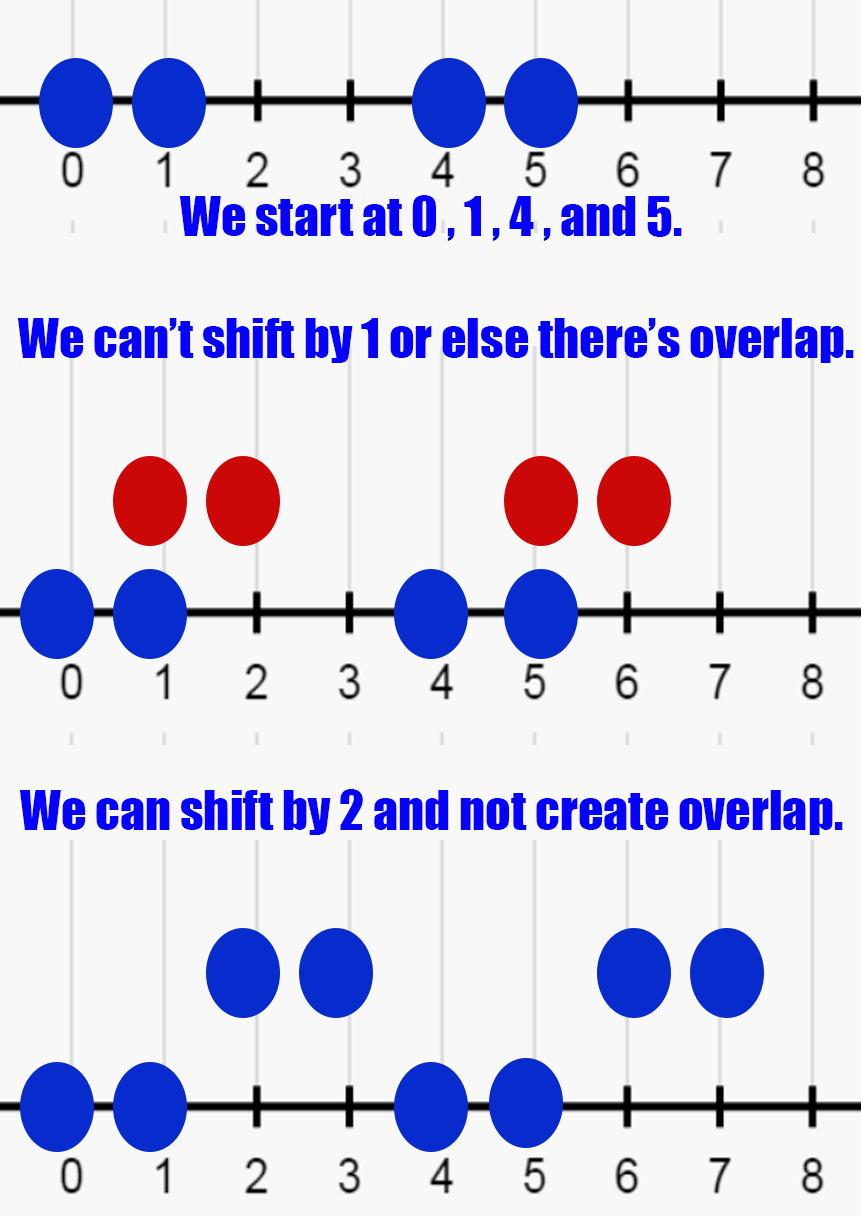
\includegraphics[scale=0.5]{numberline0145.png} \\
 \end{tabular}\\
    Look at $A = \{ 0,1,4,5 \}$. \\
 \end{center}
 
 \vspace{12pt}
 
 This $A$ has a $B$ of $ \{0,2 \}$. This makes sense because:
 \begin{itemize}
     \item We keep the initial position of the elements of $A$
     \item Shifting by one fails due to overlap.
     \item Shifting by two works and creates a consecutive string of 8 numbers.
 \end{itemize} 
 
 Incidentally, the period $N_A$ of  $A = \{0,1,4,5 \}$ is 8.
 
 
}


 
\column{.5}


\block{The Fuglede Conjecture and the Universal Tiling Conjecture in One Dimension }{
\begin{theorem*}[Fuglede Conjecture (1974)]
A domain $\Omega$ admits an operator spectrum if and only if it is possible to tile $\mathbb{R}^d$ by a family of translates of $\Omega$.
\end{theorem*}

This has been shown to be true in a variety of special cases however it has been shown to be false in both directions in dimensions 3 and higher. 
\begin{theorem*}[Universal Tiling Conjecture (Dutkay and Jorgensen, 2013)]
Let $p \in \mathbb{N}$. Let $\Gamma := {\lambda_0=0, \lambda_1,\lambda_{p-1}}$ be a subset of $\mathbb{R}$ with $p$ elements. Assume $\Gamma$ has a spectrum of the form $\frac{1}{p} A$ with $A \subset \mathbb{Z}$. Then for every finite family $A_1, A_2, ...., A_n$ of subsets of $\mathbb{Z}$ such that $\frac{1}{p} A_i$ is a spectrum for $\Gamma$ for all $i$ there exists a common tiling subset $\Tau$ of $\mathbb{Z}$ such that the set $A_i$ tiles $\mathbb{Z}$ by $\Tau$ for all $i \in \{1,....,n\}$.

\end{theorem*}

\begin{theorem*}
The following statements are equivalent.
\begin{enumerate}
    \item The Universal Tiling Conjecture is true for all $p \in \mathbb{N}$
    \item Every bounded Lebesgue measurable spectral set tiles by translations.
\end{enumerate}

Moreover, if these statements are true and if $\Omega, |\Omega |=1, $ is a bounded Lebesgue measurable set which has a spectrum with period $p$, then $\Omega$ tiles by a subset $\Tau$ of $\frac{1}{p} \mathbb{Z}$

\end{theorem*}



}

\block{Our Problem}{

Through the findings of Dutkay and Jorgensen we are able to relate these problems to statements about Fourier and Hadamard matrices. We look for two submatrices of the same Fourier Matrix that are formed from the same columns whose row sets do not share a common tiling set. This would yield a counterexample to the Universal Tiling Conjecture, in turn showing that the spectral-tile direction of the Fuglede Conjecture is false in dimension one. 

}

\block{The Generation of Hadamard Submatrices}{

We are generating our Hadamard Submatrices through a Mathematica program. It starts with a $M$ by $M$ Fourier matrix and then picks $N$ columns and rows and checks to see if the corresponding submatrix is Hadamard $H$ by examining the entries $H^*H$. If it ever fails it tries another submatrix. It at worst has an estimated run time of $O((\frac{n}{2})^2 n!)$ . 

}

\block{Newman Method}{

\begin{theorem*}
Let $a_1, a_2,...,a_k$ be distinct integers with $k=p^{\alpha}$,$p$ is a prime, $\alpha$ is a positive integer. For each pair $a_i , a_j , i \not = j$, we denote $p^{e_{ij}}$ the highest power of $p$ which divides $a_i - a_j$. The set $a_1, a_2,...,a_k$ tessellates or tiles by translation if and only if there are at most $\alpha$ distinct $e_{ij}$. 

\end{theorem*}

Invoking this theorem is a powerful tool to process a large number of submatrices. We created a program in the language C++ that properly determines if an A can tile given $|A|\leq 15$. This was a powerful tool that helped us look at some of the set of submatrices and develop intuition about tiling.


}

\block{Coven Meyerowitz (CM) Properties}{
In 1998 Ethan M. Coven and Aaron Meyerowitz discovered sufficient conditions for a set to tile. Here is some more notation that will be necessary to understand the CM Properties:

\begin{itemize}
    \item $A(x)$ is a polynomial of the form $\sum_{a \in A}x^a$ and $A(1) = |A| $
    \item $S_A$ is the set of prime powers $s$ such that $s$th cyclotomic polynomial $\Phi_s(x) $ divides A(x)
\end{itemize}

\vspace{12pt}

 \textcolor{colorTwo}{\textbf{Example:} }
 
 For $A= \{0,1,4,5 \}$, $A(x)=x^5+x^4+x+1$ and $S_A = \{2,8 \}$ \\

There are two properties need to be true in order to show that a set tiles:

\Large

\begin{itemize}
    \item[] \textbf{T1} $A(1)$ needs to equal $\prod_{s \in S_A} \Phi_s(1)$
    \item[] \textbf{T2} If $s_1,...,s_m \in S_A$ are powers of distinct primes, then $\Phi_{s_1 \cdot \cdot \cdot s_m }$ divides $A(x)$.
\end{itemize}


\normalsize

\begin{theorem*}

If $|A|$ has at most two prime factors, then $A(x)$ satisfies the two CM Properties if and only if $A$ tiles the integers. 

\end{theorem*}

The CM Properties check have been implemented in our C++ program to allow us to check if all the submatrices in our data actually tile. 

}


\column{.25}
\block{Determining Period and Tile Set of $A$}{

Coven and Meyerowitz also found that the period and tile set of $A$ can be determined through use of $A(x)$ and $S_A$. The period is defined to be the least common multiple amongst all of the elements of $S_A$. Finding $B$ is slightly more difficult. First we must define $B(x)$ to be \[\prod \Phi_{s_B}(x^{t(s_B)}), \] where $s_B $ range over the prime power factors of $N_A \not \in S_A$ and $t(s_B)$ is the largest factor of $N_A$ relative prime to $s_B$.\\

\textcolor{colorTwo}{\textbf{Example:} }
 Let's look at $A = \{0,1,4,5 \}$ again.
 
 Its $S_A = \{ 2,8 \}$. The period $N_A$ is $lcm(2,8)=8$, and $B(x)$ is $\Phi_{4}(x^{1}) = x^2+1 $ because our only $s_B $ is $4$ which only has $1$ as a relatively prime factor to $8$. This confirms that the tiling set $B = \{0,2\}$ as we showed earlier by hand. \\
 
 This method is very applicable and useful in testing large numbers of submatrices. 

}

\block{Results}{
We have found that for all of the Hadamard submatrices from $\mathcal{F}_{2}$ up to $\mathcal{F}_{18}$ do tile. All of the rows that have a common column set have the same period. However, there can be multiple 
periods amongst the same size of Hadamard submatrices generated from the same Fourier Matrix. 

}
\block{Further Study}{
We have developed multiple goals to help guide this project further:
\begin{itemize}
  \item Determine the tiling set of all our current submatrices.
  \item Write the Hadamard Submatrix Generator in a less interpreted language that can be run in parallel (C++) to be able to gather more submatrices to analyze
  \item Increase the capacity of the Tiling Check Program to handle larger submatrices when they are produced.
  \item Discover a technique to check for set sizes of three or more distinct prime powers.
\end{itemize}

}
\block{References}{

\begin{itemize}
    \item Bond, Bailey, Glickfield, Alexander, and Herr, John E. (2018). On the Existence of Complex Hadamard Submatrices of the Fourier Matrices.
    \item Dutkay, Dorin & Jorgensen, Palle. (2012). On the Universal Tiling Conjecture in Dimension One. Journal of Fourier Analysis and Applications.
    \item Dutkay, Dorin & Kraus, Isabelle. (2018). On spectral sets of integers. Contemporary Mathematics. 215-234.
    \item M. Coven, Ethan & Meyerowitz, Aaron. (1998). Tiling the Integers with Translates of One Finite Set. Journal of Algebra. 212.
    \item Newman, David. (1977). Tesselation of integers. Journal of Number Theory - J NUMBER THEOR.
\end{itemize}

}
\end{columns}

\end{document}









